
\section{Methods Supplemental Information}


\subsection{Experimental Procedures}

\subsubsection{Test Case Sequences}

%Probably should define acronyms again in SI the first time they are used.
%MWT, SFW, SFR

Throughout the experimental campaign, we performed the following test case sequences. The test cases are presented below with our internal naming scheme that begins with a three digit number that represent the nominal values for the HVOF process inputs. The first digit represents the total mass flow (5 = 13.0 g/s), the second digit represents the equivalence ratio (1 = 0.6, 3 = 0.8), and the third digit represents the potassium mass fraction (3 = 0.1\% and 6 = 1.0\%). A 'x' indicates that the nominal value was varied during that sequence. The sequence is then appended with 'pos' or 'pow' to indicate a position or power sweep, respectively. The absence of 'pos' or 'pow' indicates that the SFR-maximized position of 180mm downstream of the barrel exit and full laser power (7 mJ) were used. A given test case sequence is appended with a 'run number' to indicate repeats of the sequence performed on the same day. 

%Define Kwt here? Is it defined differently in main text?
\begin{itemize}
    \item 536 Position: Varying motorized stage position. Full laser power. Kwt = 1\%, phi = 0.8 (presented in main text). Performed on 2023-04-07, 2023-05-12, 2023-05-18.
    \item 516 Position: Varying motorized stage position. Full laser power. Kwt = 1\%, phi = 0.6 (presented in main text). Performed on 2023-05-24.
    \item 53x: Varying potassium mass fraction. Motorized stage at SFR-maximized position. Full laser power. (presented in main text). Performed on each date. 
    \item 536 Power: Varying laser power. Motorized stage at SFR-maximized position. Kwt = 1\%. Performed on each date. 
    \item 5xx: Varying potassium mass fraction and equivalence ratio. Motorized stage at SFR-maximized position. Full laser power. Performed on 2023-05-24.
    \item 5x6\_pos/5x3\_pos: Varying motorized stage position and equivalence ratio. Full laser power. Kwt = 0.1\% or 1\%. Performed on 2023-05-24.
\end{itemize}

For each diagnostic, data is obtained continuously throughout the experiment and indexed in time. For each individual test case, there are a number of repeated acquisitions depending on the duration of the test case and acquisition rate of the diagnostic. In the data processing, these repeated acquisitions are averaged to obtain a single value for each test case before further analysis (e.g. fitting). For statistics across runs presented in the main text, the variation within repeat acquisitions is not considered. 

The syringe pump limits the duration of a given test case sequence, with shorter durations at high potassium mass fraction. Furthermore, it was not possible to maintain consistent durations for the same test cases performed in different sequences.
The time limitation on seeding duration limits the AES diagnostic more than the MWT diagnostic. The AES diagnostic must wait 1 second between LED switching events to allow for the LED to stabilize. Additionally, the multiplexer switches every 10s. Therefore a minimum of at least 20 s is needed for a nK measurement at both location, but ideally multiple measurements are taken at each location to ensure reproducibility. The MWT diagnostic, on the other hand, is continuously acquiring at the repetition rate of the laser (5-12 Hz).  Therefore for a given test case sequences, the MWT diagnostic has more data than the AES diagnostic. For the standard test case sequences outlined above, approximately 1 minute was used for each test case and data is presented for both diagnostics.




\subsubsection{Experiment Overviews}

Below are overviews of the experiments performed. The independent variables that were varied throughout the experiments are shown and the colored regions are test case sequences. Times are in PST. Note that not all test case sequences that were performed were analyzed in the main text. 


\foreach \date in {2023-04-07, 2023-05-12, 2023-05-18, 2023-05-24}{
    \begin{figure}[h]
        \centering
        \includegraphics[width=0.9\linewidth]{\repodir/experiment/analysis/auto/output/figures/tc_plot_\date.png} 
        \caption{Experiment Overview for \date. The colored regions are test case sequences.}
        \label{fig:SI_expt_overview_\date}
    \end{figure}

    \begin{figure}[h]
        \centering
        \includegraphics[width=0.9\linewidth]{\repodir/experiment/analysis/auto/output/figures/other_signals/tc_plot_\date.png} 
        \caption{Additional signals for \date. The colored regions are test case sequences with the same scheme as in \ref{fig:SI_expt_overview_\date}.}
        \label{fig:SI_expt_overview_other_\date}
    \end{figure}

}

\clearpage

\subsection{Data Pipeline}

The results of this work are created from a set of codes located at \url{https://github.com/MHDLab-Projects/MHD-Photoionization}. The final results and figures are the output of a data pipeline.  The data pipeline starts from the raw experimental dataset, which consists of unprocessed data taken during the experiments. The data pipeline consists of a series of shell scripts that in turn primarily run python scripts. Therefore, the shell scripts in the repository can act as a map of the data processing methodology. The data pipeline has the following steps: 

\begin{enumerate}
    \item Data Munging (\texttt{/automation/munge.sh}): The raw data is initially processed to reduce the size of the dataset and to convert the data to common formats of either "tdms" (National Instruments) or "cdf" (xarray python package). This includes the standard data processing steps of our lab for time series data (located in /PostProcessor), which most notably includes resampling from the 1 kHz data acquisition rate to one sample per second. Additionally, resampling and combining of individual acquisition files is done for the MWT oscilloscope data.  At this stage, the data collected during each experiment is processed separately.
    \item Process Munged Data (\texttt{/automation/process\_munged.sh}): Data is combined from different dates to create single datasets for each diagnostic. Then, test case time windows are used to create datasets for the test case sequences, with the independent variables (Potassium mass fraction, equivalence ratio, stage position, laser power, experiment date, run number, acquisition number) being added as coordinates in xarray datasets.
    \item Create Final Dataset (\texttt{/automation/final\_dataset.sh}): The final dataset is created by applying various analysis steps (data extraction, fitting, etc.) to the processed data. 
    \item Generate Figure Panels (\texttt{/automation/gen\_fig\_panels.sh}): The final dataset is used to generate the figure panels (A, B, C, etc.)for the main manuscript. 
    \item Render Figures (\texttt{/automation/render\_figures.sh}): The figure panels are combined into the final figures for the manuscript. The figures panels are laid out in SVG files, and the SVG file is rendered with Inkscape to create the final figure PNG file. 
\end{enumerate}

In addition to the above steps that lead to the final figures, the repository contains a variety of analysis scripts that contain supplemental/exploratory figures that were generated throughout the data analysis process. These scripts are rendered as jupyter notebooks in a subfolder called "nb\_render", relative to the analysis script. These notebooks are collected and rendered to PDFs in final/output/nb\_renders. 

The supplemental analysis scripts need to be run to generate the supplemental figures. The shell commands \texttt{automation/render\_all\_expt.sh} and \texttt{automation/render\_all\_expt.sh final} will render these scripts to Jupyter notebooks 'renders'. During this process many of the supplemental figures are created, though those figures could also be generated running the scripts directly. Finally, there are scripts not automated in the above process that contain some supplemental figures, which are outlined in \texttt{automation/supp\_scripts.sh}. 

Figure \ref{fig:SI_Data_Processing_Simple} shows an overview of the data processing pipeline.

\begin{figure}[H]
\centering
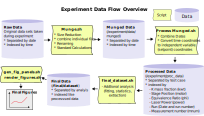
\includegraphics[width=0.8\textwidth]{\repodir/final/figures/schematics/output/Data_Processing_Simple.png}
\caption{Overview of the data processing pipeline.}
\label{fig:SI_Data_Processing_Simple}
\end{figure}


\clearpage
\subsection{Microwave Transmission (MWT)}


\subsubsection{Setup Description}
\begin{figure}[]
\centering
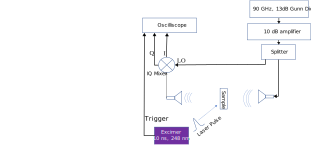
\includegraphics[width=0.8\textwidth]{\repodir/final/figures/SI/output/MWT_Setup.png}
\caption{Microwave transmission setup. Left: An image of the setup. Right: A schematic of the setup. LO: local oscillator. I: In-phase. Q: Quadrature.  }
\label{fig:SI_MWT_Setup}
\end{figure}

The microwave transmission setup (MWT) is shown in Figure \ref{fig:SI_MWT_Setup}. The parts used to construct this setup were ordered from Erevant, formerly Sage Millimeter. The system is W-band and based on WR-10 waveguides. The microwave source is a \SI{90}{\giga\hertz} Gunn oscillator (SOM-90305213-10-S1) with an output power of +13 dBm. The output of this source is fed into a 10 dB gain, 15 dBm P1dB in-line waveguide power amplifier (SBP-7531141015-1010-E1). The output of the power amplifier is then fed into a 4-way in-line power divider (SWP-90310404-10-E1). In the current configuration, only two outputs of the power divider are used, and the remaining two are terminated with waveguide terminators (SWL-1027-S1). One leg of the power divider is used for the main transmitted power, which is sent through waveguides to a rectangular horn antenna (SAR=2013-10-S2) that transmits the microwaves into free space. The transmitted microwaves, which have passed through the sample, are collected by the same type of horn, and the collected microwaves are sent to the IQ mixer (SFQ-75311415-1010SF-N1-M). The LO input of the IQ mixer is fed by the remaining port of the power divider. 

% Between the power divider and the LO input there is a phase shifter (STP-18-10-M2) that is typically used to maximize the I signal in the absence of a sample. 

The I and Q signals from the oscilloscope are fed directly into a Teledyne Lecroy WavePro 404HD-MS Oscilloscope.  The oscilloscope is triggered from the excimer laser. 

The oscilloscope was used with a \SI{1}{\mega\ohm} input impedance with DC coupling for the I/Q signals, and \SI{50}{\ohm} input impedance for the photodiode signals. The vertical coupling was \SI{20}{\milli\volt/div} on 2023-04-07 and 2023-05-12, and \SI{50}{\milli\volt/div} on 2023-05-18 and 2023-05-24 for the IQ signals. There was an increased signal intensity on the second two dates, which we attribute to cleaning of residue from the microwave horns, as discussed in Sec.\ \ref{sec:no_torch_measurements}. The vertical coupling of the photodiode signals was \SI{20}{\milli\volt/div} for on-peak, and \SI{10}{\milli\volt/div} off-peak. The horizontal coupling was \SI{10}{\micro\second/div}.

The excimer laser was used with 12 kV pulse power. The repetition rate of the laser varied: 2023-04-07 5Hz, 2023-05-12: 12 Hz, 2023-05-18: 5 Hz, 2023-05-24: 5 Hz. The oscilloscope was used with no averaging of acquisitions, with a file saved for each acquisition. The repetition rate was limited by the rate at which the oscilloscope could save individual files to disk. 

The excimer laser is sent through a 90/10 UV beam splitter with the 10 \% sent to a photovoltaic power meter (Ophir PD-10C). There is an iris with a \SI{2.7(0.05)}{\milli\meter}  opening before a UV enhanced neutral density filter with optical density of 3 before the power meter. The power data was not used in this analysis but is present in the dataset. The remaining 90 \% of the laser is directed through a Thorlabs FW 102C filter wheel. The filter wheel housed Thorlabs reflective UV neutral density filters. These neutral density filters have been observed to degrade from continued use with the excimer laser, and the laser power was measured before an after the experiment to ensure there was no significant degradation in filter performance. After the filter wheel, the laser is redirected with a UV mirror (Acton Instruments, 248-FR45-ID-MB) to the center of the microwave horns. Everything including the final mirror is located on the motorized stage, which moves parallel to the torch axis. 

The distance between the horns is \SI{85.725}{\milli\meter}. The mirror that sends the excimer beam to the measurement location is located \SI{247}{\milli\meter} downstream along the torch axis, \SI{397}{\milli\meter} horizontally (along the table) perpendicular from the torch axis, and \SI{65}{\milli\meter} vertically above the torch axis. 


\subsubsection{Data Processing and Fitting}

The raw MWT data consists of individual files containing channel time traces, and each raw data file corresponds to an individual laser pulse. No averaging of multiple laser pulses occurs before the data is saved to disk. While the data is writing to disk, laser pulses can be missed. After 2023-05-12, the pulse rate was limited to \SI{5}{\hertz} to minimize this effect. 

The MWT data is first munged by combining all individual "acquisitions" files into a single dataset with a common oscilloscope time axis. To reduce the size and processing time of this dataset, the data is resampled. Within the region of \SI{700}{\nano\second} to \SI{1500}{\nano\second} (the laser pulse is at approximately \SI{800}{\nano\second}, see Figure 2 in the main text) the data is resampled by grouping data points into groups of 10 and averaging. Outside this region, the data is grouped into \SI{1000}{\nano\second} data points and averaged. The effect of this resampling can be seen in Figure \ \ref{fig:SI_mwt_resampling}

\begin{figure}
\centering
\includegraphics[width=0.8\textwidth]{\repodir/experiment/analysis/mwt/resampling/output/figures/mwt_sample_nors_compare.png}
\caption{Comparison of the resampling methods. Both left and right panels show the same time trace, with the right panel being zoomed into the peak.}
\label{fig:SI_mwt_resampling}
\end{figure}

Figure \ref{fig:SI_mwt_processing_overview} shows the following processing steps performed on the MWT data, which we use to determine the $\Delta AS$ profiles, as described in the main text. The resulting $\Delta AS$ data is down selected to a window of \SI{5}{\micro\second} to \SI{20}{\micro\second} after the laser pulse and fit with an exponential fit model $y = A \exp(-t/\tau) $.


\begin{figure}[]
\centering
\includegraphics[]{\repodir/experiment/analysis/mwt/output/figures/mwt_processing_overview.png}
\caption{Microwave processing overview. From top to bottom: A) raw I and Q signals. B) the calculated magnitude (U) C) The Transmission (T). D) Absolute absorption and scattering (AS). See main text for formulas and term definitions.  }
\label{fig:SI_mwt_processing_overview}
\end{figure}


\subsubsection{No-Torch Measurements} %"Sans-Torch measurements"?
\label{sec:no_torch_measurements}

On each date, the microwave transmission magnitude with nothing in between the horns, $U_{0}$, was measured. During these measurements, all other settings are the same (excimer laser, oscilloscope, etc.) compared to the main experimental measurements.

An example measurement of $U_{0}$ is shown in Figure \ref{fig:SI_MWT_nothing_time_trace}. For approximately 1 $\mu s$ there is electronic interference from the laser pulsing, which also appears in the main experimental transmission measurements. 



\begin{figure}[]
\centering
\includegraphics[]{\repodir/final/dataset/output/figures/mwt_nothing_time_trace_2023-05-18.png}
\caption{Time trace from 2023-05-18 of the transmission measurement without any free jet. The time has been shifted by an offset of \SI{880}{\nano\second} to align the laser pulse to t=0.}
\label{fig:SI_MWT_nothing_time_trace}
\end{figure}

On 2023-05-24 $U_{0}$ was measured as a function of position as shown in Figure\ \ref{fig:SI_MWT_nothing_motor}. There is a slight increase in transmission when the stage is moved as close as possible to the barrel exit, possibly due to reflections from the barrel.


\begin{figure}
\centering
\includegraphics[]{\repodir/final/dataset/output/figures/mwt_nothing_motor_2023-05-24.png}
\caption{Motorized stage for position dependent transmission measurements.}
\label{fig:SI_MWT_nothing_motor}
\end{figure}


The $U_{0}$ measured at the SFR-maximized position (\SI{180}{\milli\meter} downstream from barrel exit) for each of the dates is presented in \ref{fig:SI_MWT_nothing_T0}A. Note that for 2023-05-12, $U_{0}$ was only taken at the barrel exit, which is corrected by a factor of 0.95 to calculate $U_{0}$ at the SFR-maximized position for that date. This factor is determined from the ratio of the transmission at the SFR-maximized position to the transmission at the barrel exit from Figure \ref{fig:SI_MWT_nothing_motor}. Figure \ref{fig:SI_MWT_nothing_T0}B shows the magnitude of absolute transmission (see equation for $T$ in main paper) of the seeded torch before the laser pulse for the case 536\_pos, taken on multiple dates. 

On 2023-05-18, a blue residue/corrosion was found in the waveguides, possibly from a chemical reaction or deposition from the seeded free jet. The microwave horns were cleaned and other waveguide parts were replaced. This change could explain the increased $U_{0}$ on 2023-05-18 and 2023-05-24.



\begin{figure}[]
\centering
\includegraphics[width=0.8\textwidth]{\repodir/final/analysis/mwt/output/figures/mwt_nothing_T0.png}
\caption{ From left to right: A) Measurement of transmission without any torch at a position of 180 mm (except 2023-05-12, as described above) B) position-dependent transmission measurements.}
\label{fig:SI_MWT_nothing_T0}
\end{figure}

\subsubsection{Silicon test sample}

Before each experiment, we performed measurements with a silicon sample in the location of the torch to ensure the system was functioning properly. The silicon wafer was ordered from MTI corporation (Item Number: SIUa50D05C1R1000) and has the properties shown in Table \ref{table:material_properties}.

\begin{table}[h]
\centering
\begin{tabular}{|l|l|}
\hline
Property & Value \\
\hline
Single crystal & Si \\
Conductive type & N type, undoped \\
Resistivity & > \SI{1000}{\ohm\centi\meter} \\
Size & 2 inch diameter x \SI{0.5}{\milli\meter} \\
Orientation & (100) \\
Polish & one side polished \\
Surface roughness & < \SI{5}{\angstrom} RMS \\
\hline
\end{tabular}
\caption{Properties of the test silicon wafer}
\label{table:material_properties}
\end{table}

The silicon measurements are shown in \ref{fig:SI_MWT_Silicon}. The measured exponential time constant is consistent with the minority carrier lifetime in an undoped silicon wafer. \cite{tyagiMINORITYCARRIERRECOMBINATION, delalamoModellingMinoritycarrierTransport1987} %missing citation

\begin{figure}[]
\centering
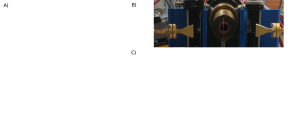
\includegraphics[width=0.8\textwidth]{\repodir/final/figures/SI/output/MWT_Silicon.png}
\caption{Measurements of the MWT system with a Silicon sample. A) Power dependent measurements of I, Q, and the calculated magnitude $U$. B) a picture of the silicon sample placed in the location of the torch. C) the $\Delta AS$ curve for the silicon sample with an exponential fit. }
\label{fig:SI_MWT_Silicon}
\end{figure}

\clearpage
\subsubsection{Laser Profile and Power}

The laser profile was measured by terminating the laser beam on a white Thorlabs beam block and imaging with a Thorlabs DCC1240C-HQ camera. The images are shown in Figure \ref{fig:SI_Laser_Profile}A. Cross-sections of this image are taken to obtain the full width at half maximum (FWHM) of the laser profile and calculate the area of the beam. 

\begin{figure}[H]
\centering
\includegraphics[width=0.8\textwidth]{\repodir/experiment/analysis/mwt/output/figures/laser_profile.png}
\caption{Laser profile measurement. Left to Right: A) The image of the laser profile. B) The cross-sections of the laser profile. The width of the cross-sections and calculated area are indicated in the figure.}
\label{fig:SI_Laser_Profile}
\end{figure}

%above figure has no A or B label

The laser power was measured with an Ophir PE25BG-C pyroelectric power meter before and after the experiments as shown in Figure \ref{fig:SI_Laser_Energy} 



\begin{figure}[H]
\centering
\includegraphics[]{\repodir/experiment/analysis/various/output/figures/laser_energy_date.png}
\caption{Measurement of the laser pulse energy. The data points include measurements before and after the experiment. The average laser power across all measurements is shown in the figure title. }
\label{fig:SI_Laser_Energy}
\end{figure}


\subsubsection{Mie Scattering Analysis}

To examine the relative contributions of absorption and scattering of microwaves on our transmission signal, we examined models of Mie scattering of a weakly conducting sphere of air plasma. Mie scattering refers to the scattering or absorption of electromagnetic radiation by a sphere of objects with a size that is comparable or larger than the wavelength of incident radiation \cite{bohrenAbsorptionScatteringLight2007}. We model our laser-plasma interaction volume as a sphere, for which analytical expressions exist for the absorption efficiency, $Q_{abs}$, and the scattering efficiency, $Q_{sca}$. The diameter of the sphere is \SI{10}{\milli\meter} and the radiation wavelength is \SI{3}{\milli\meter}, which are approximately the diameter of our laser beam and wavelength of our \SI{90}{\giga\hertz} microwave source, respectively.  %broken citation

$Q_{abs}$ and $Q_{sca}$ are defined through $Q_x = \frac{\frac{P_x}{I}}{A_p}$, where $I$ is the incident radiation, $A_p$ is the particle cross-sectional area, and $P_x$ is the power with $x=abs$ and $x=sca$ corresponding to absorbed or scattered radiation, respectively \cite{bohrenAbsorptionScatteringLight2007}. The extinction efficiency is defined as $Q_{ext} = Q_{abs} + Q_{sca}$, which will be related to the measured power transmission. %broken citation

%preference on using "Fig." or "Figure" when it appears in the middle of a sentence? %LA: Fig. changed to Figure

We use the python package PyMieScatt to determine the various efficiencies, $Q$, as a function of the imaginary permittivity, $\epsilon_i$, as shown in Figure \ref{fig:SI_Mie_Scattering}A. $\epsilon_i$ is related to the electrical conductivity, $\sigma$, through $\epsilon_i = \sigma/\omega$, where $\omega$ is the frequency of radiation.\cite{coltonComplexWaveNumber2021}  We model the complex index of refraction, $\epsilon$, as $\epsilon = 1 + i\epsilon_i$. We double-check correct use of the analytical expressions by performing 3D finite-difference time-domain (FDTD) simulations of transmission through a sphere and measuring the transmission directly, also shown in Figure \ref{fig:SI_Mie_Scattering}. It can be seen that as $\epsilon_i \rightarrow 0$, $Q_{ext}$ becomes dominated by $Q_{abs}$, indicating that absorption is the primary mechanism by which radiation transmission is reduced in the low conductivity regime relevant for exponential decay (see main text MWT section or Equation \ref{eq:ne_exp_decay}).

In Figure \ref{fig:SI_Mie_Scattering}B, we perform a power-law fit of $Q_{ext}$ for small $\epsilon_i$, and determine an exponent approaching 1, indicating the relationship that $Q_{abs} \propto \sigma$. 


\begin{figure}[H]
\centering

\includegraphics[width=0.8\textwidth]{\repodir/final/figures/SI/output/MieScatt.png}
\caption{Analysis of Mie Scattering. A) The absorption, scattering, and extinction efficiencies as a function of the imaginary permittivity, $\epsilon_i$. B) The extinction efficiency as a function of $\epsilon_i$ for small $\epsilon_i$. The power law fit is shown in the figure.}
\label{fig:SI_Mie_Scattering}
\end{figure}


%OK to include package csquotes to fix backwards ’ ’ quotes? %LA: yes
In Figure \ref{fig:SI_MWT_lin_square_compare}, we compare the transmission calculated from the microwave signal magnitude ($U$) squared, as done in the paper ($T_{square}  = \frac{U^2 - U_{block}^2}{U_0^2 - U_{block}^2}$) with the same expression without squaring the magnitude ($T_{linear}  = \frac{U - U_{block}}{U_0 - U_{block}}$), where $U_0$ and $U_{block}$ are the magnitude with no object and with blocked receiver. The exponential decay time of $\Delta AS$ can be seen to be invariant to whether power or magnitude transmission is used for calculation. 

%TODO: Spell check throughout 

\begin{figure}[H]
\centering

\includegraphics[width=0.8\textwidth]{\repodir/final/figures/SI/output/MWT_lin_square_compare.png}
\caption{Comparison of the transmission calculated from the microwave magnitude ($U$) A) squared (as in main text) and B) not squared (linear)}
\label{fig:SI_MWT_lin_square_compare}
\end{figure}


\clearpage
\subsection{Absorption Emission Spectroscopy (AES) Setup}

\subsubsection{Setup Description}

The LED used for AES is a Thorlabs M780F2 \SI{780}{\nano\meter} LED driven by a Thorlabs T-Cube LED Driver with input current set to approximately \SI{0.6}{\ampere}. The LED is fed into a Thorlabs M28L02 fiber with \SI{400}{\micro\meter} diameter and 0.39 NA. The fiber is then connected to the input of an Ocean Optics MPM-2000-UV-VIS600-2X8 Multiplexer. The multiplexer can send light to either of the AES locations (barrel exit and mobile stage). The multiplexer continuously switches between the two AES locations every \SI{10}{\second} throughout the duration of an AES measurement. After collection of light with the collection lenses (as described below), the light collected from both the barrel exit and the translation stage is sent back to the multiplexer. Finally, the light is routed from multiplexer to the spectrometer through an Ocean Optics QP-600-2-VIS-NIR fiber. Because both AES locations are multiplexed to the same spectrometer, the measurements at the two AES locations are not simultaneous.

For the barrel exit measurement, the light from the LED is collimated from the fiber with a RC02SMA-P01 reflective parabolic mirror and directed at a \SI{90}{\degree} angle with a MRA05-E3 dielectric mirror. After passing through the torch, the light is then coupled into the collecting fiber with a second RC02SMA-P01 reflective parabolic mirror. The light is sent from the multiplexer to the collimating lens with a Thorlabs M38L02 \SI{200}{\micro\meter} 0.39 NA fiber, and sent from the collection lens to the multiplexer with a Thorlabs M53L02 \SI{600}{\micro\meter} 0.5NA fiber. On both sides of the torch, light passes through an iris of approximately \SI{1}{\milli\meter} and a glass slide which is used to protect the optics from the torch. The beam is positioned to go through the center of the torch at approximately 1/8 inch \pm 1/16 inch downstream of the barrel exit. The beam diameter is approximately 3/32 inch to 4/32 inch. 

For the mobile absorption measurement, the light is collimated and collected with Thorlabs F950SMA-A multimode collimating lenses. On the collection side, there is a 3.25 \pm 0.5 iris. The light is sent from the multiplexer to the collimating lens with a Thorlabs M28L02 400um 0.39 NA fiber, and sent from the collection lens to the multiplexer with a Thorlabs M53LO2 600 um 0.5 NA fiber. 

The LED is continuously turned on and off throughout the experiment to obtain "LED on" and "LED off" measurements. The LED is triggered by the spectrometer. When switching the LED, there is a \SI{1}{\second} delay before the spectrometer is triggered to allow the LED state to stabilize. This LED switching time limits the temporal resolution of the AES measurements. 

\subsubsection{Data processing and Fitting}

Figure \ref{fig:SI_AES_proc_overview} shows the processing steps for the AES data.


\begin{figure}[]
    \centering
    \includegraphics[height=0.6\textheight]{\repodir/experiment/analysis/absem/output/figures/absem_proc_overview.png}
    \caption{AES processing overview: A) LED on and off measurements. B) Difference (LED on - LED off) compared to the interpolated calibration measurement. C) Absorption calculation (raw) and absorption after offset removal. D) Fitted absorption profile (Data) and fit.}
    \label{fig:SI_AES_proc_overview}
\end{figure}


Before and after each experiment, calibration spectra are taken with no free jet in place. The calibration is required to determine the absorption $\alpha(\lambda)$, as described in the main text.  The calibration spectra are derived from the difference between the "LED on" and "LED off" measurements (similarly to the absorption data). For the position dependent measurements, the calibration spectra are taken at the SFR-maximized position. 

%DN: Is the SFR-maximized position always 180 mm, as mentioned previously? If so, for clarity we should say "SFR-maximized position (180 mm from the barrel exit)" every time "SFR-maximized position" is used %LA: SFR-maximized clarified on first use (also defined in main text)

We observe changes in the calibration spectra throughout the experiment which cause offsets in $\alpha(\lambda)$. Unfortunately, the calibration spectrum cannot be obtained throughout the experiment as turning off and restarting the HVOF torch is unreliable, so we elect to run the torch continuously through each experiment. We develop a method to correct the calibration spectra using the "LED on" and "LED off" measurements. Figure \ref{fig:SI_absem_calib_dates} shows the calibration spectrum for each date. For the current work, we interpolate the calibration spectra shown in figure \ref{fig:SI_absem_calib_dates} to the time of any given measurement to determine the calibration spectrum for that measurement. 

\begin{figure}[]
    \centering
    \includegraphics[width=0.8\textwidth]{\repodir/experiment/analysis/absem/output/figures/absem_calib_dates.png}
    \caption{Calibration spectra taken at different time on different dates. }
    \label{fig:SI_absem_calib_dates}
\end{figure}

%DN: Ideally, wouldn't switch between saying "absorption" and $\alpha(\lambda)$. But I'm not certain whether "absorption" can always be replaced with \alpha, and if "absorption spectrum" can always be replaced with $\alpha(\lambda)$. 

Even with interpolation, slight differences between the calibration spectrum and off-peak free-jet $\alpha(\lambda)$ measurements are observed. For some measurements, this offset is different on either side of the peak in $\alpha(\lambda)$ (see Figure \ref{fig:SI_5x3_pos_alpha}). The cause of this asymmetric offset is unknown, and we have not developed a method to correct for asymmetric offsets. For constant offsets, we perform an offset procedure that maintains the overall shape of $\alpha(\lambda)$ near the high limit of the absorption data (i.e. the offset removal does not affect $\alpha$ values near 1). The offset procedure is as follows:

\begin{enumerate}
    \item Calculate $\beta = -\ln(1 - \alpha)$, which represents the exponential component of the Beer-Lambert law. 
    \item Subtract an offset $\beta$, $\beta{off}$, which is the average of $\beta$ in a region of 750 to 755 nm where the $\alpha(\lambda)$ is expected to be zero. 
    \item Recalculate $\alpha = 1 - e^{- (\beta - \beta_{off})}$ 
\end{enumerate}

The effect of the offset procedure is shown in Figure \ref{fig:SI_AES_proc_overview}C. Additional processing steps are as follows:

\begin{enumerate}
    \item Individual acquisitions with a negative absorption in the 765 to \SI{772}{\nano\meter} range are removed. Negative absorption can occur when there is a significant fluctuation in seed level between the LED on and LED off measurements.
    \item The data is reduced to the wings of the absorption profile. From the left and right of the spectrum, the data is kept until a point where the absorption is 0.8. This avoids fitting where the absorption is near 1. 
    \item All individual acquisitions for a given test case are averaged.
\end{enumerate}

We model $\alpha(\lambda)$ to determine the centerline potassium density, $n_{K,max}$, by numerically integrating the Beer-Lambert law along the path $s$ of the beam for the wavelength-dependent intensity, $I(\lambda)$

\begin{equation}
    \frac{dI}{dx}(\lambda) = -\mu_{atten}(\lambda, s) I(\lambda)
\end{equation}

Where $\mu_{atten} (\lambda, s)$ [1/cm] is the attenuation coefficient, which is given by 

\begin{equation}
    \mu_{atten}(\lambda, s) = -\kappa(\lambda) n_{K,max} f_{K, CFD}(s),
\end{equation}
where $\kappa(\lambda) [cm^2]$ is the absorption cross-section, $n_{K,max}$ is the maximum potassium number density, and $f_{K, CFD}(s)$ is the profile of the potassium number density along the beam path determined by CFD. The $f_{K, CFD}(s)$ profiles are extracted along a line perpendicular to the torch axis for the barrel exit measurements, and along the beam path (ratio of 1.875:4.25 parallel and perpendicular to the torch axis, respectively) for the mobile measurements. The CFD profiles are shown in Figure \ref{fig:SI_cfd_beam_goldi_pos_kwt} and Figure \ref{fig:SI_cfd_beam_pos_dep}.

The fitting procedure is as follows:


\begin{enumerate}
    \item A profile of the potassium atom density from the CFD data along the beam path is obtained, as shown in Figures \ref{fig:SI_cfd_beam_goldi_pos_kwt} and \ref{fig:SI_cfd_beam_pos_dep}. This profile is normalized to the maximum value to give $f_{K, CFD} (s)$. $s$ represents the distance along the beam path.
    \item The potassium atom density profile is converted to $\mu_{atten} (s, \lambda) = n_{K,max}* f_{K, CFD} (s) \kappa(\lambda)$. $n_{K,max}$ is the fit parameter corresponding to the centerline (maximum) potassium atom density in the profile.
    \item For each $\lambda$, the intensity profile $I(s)$ is calculated along the beam path with the Euler method: $I(s + \Delta s) = I(s) + \mu_{atten}(s, \lambda) I(s) \Delta s$. The initial condition is $I(0) = 1$. If the intensity becomes negative, the calculation is stopped and the absorption is set to 1. An example of the Euler method is shown in Figure \ref{fig:SI_euler_method_tophat_demo}.
    \item The absorption is calculated as $\alpha(\lambda) = 1 - I(s_{max})$, where $s_{max}$ is the maximum distance along the beam path. 
    \item The spectrometer has a finite resolution that "blurs" the input light spectrum across the spectrometer CCD pixels. We model this effect by applying a Gaussian filter to the final absorption profile $\alpha(\lambda)$ with a Gaussian width of \SI{0.026}{\nano\meter}. The data is first interpolated to a grid with \SI{0.026}{\nano\meter} spacing before the Gaussian filter is applied, then the data is interpolated back to the original grid.
\end{enumerate}

$\kappa(\lambda)$ is modeled as a sum of two Voigt line profiles, following Bedeck et al.\cite{bedickDeterminationElectricalConductivity2019} and is converted to a wavelength basis with the relationship $\Delta \lambda/\lambda_0 = \Delta \nu/\nu_0$, where $\Delta \lambda$ is the width of the line in wavelength space, $\Delta \nu$ is the width of the line in frequency space, $\lambda_0$ is the central wavelength of the line, and $\nu_0$ is the central frequency of the line. $\kappa(\lambda)$ is given by %DN: Broken citation

\begin{equation}
    \label{eq:cross_section_alpha_fit}
    \kappa(\lambda) = \frac{e^2}{4 \epsilon_0 m_e c^2} \left[ \frac{4}{6} f_1 \lambda_{0,1}^2 V(\lambda_{0,1},\sigma,\gamma_1) + f_2 \lambda_{0,2}^2 V(\lambda_{0,2},\sigma,\gamma_2) \right],
\end{equation}

%TODO: Check all mentions of Gaussian to make sure they are capitalized
where $f_i$ is the oscillator strength of the i\textsuperscript{th} peak, $\lambda_{0,i}$ is the central wavelength of the i\textsuperscript{th} peak, and $V(\lambda_{0,i},\sigma,\gamma_i)$ is the Voigt profile. The two parameters for the Voigt profile are the Gaussian width converted into a wavelength basis, $\sigma_i = 2*\sqrt{2*ln(2)*k_b*T/m_K}*(\lambda_{0,i}/c)$, and the Lorentzian width $\gamma_i = (\lambda_i^2/c)*\Delta \nu_{i,C}$, where $\Delta \nu_{i,C}$ is the collisional broadening frequency width of the peak, $T$ is the temperature, $m_K$ is the atomic mass of potassium, $k_b$ is the Boltzmann constant, and $c$ is the speed of light. The parameters used for each peak are shown in Table \ref{table:peak_parameters}. 

\begin{table}[H]
\centering
\begin{tabular}{|c|c|c|}
\hline
Parameter & Peak 1 & Peak 2 \\
\hline
Oscillator strength ($f_i$) & 0.7 & 0.35 \\
Central wavelength ($\lambda_{0,i}$) & \SI{766.504}{\nano\meter} & \SI{769.913}{\nano\meter} \\
Collisional frequency width ($\Delta \nu_{i,C}$) & \SI{3.19}{\giga\hertz} & \SI{3.04}{\giga\hertz} \\
\hline
\end{tabular}
\caption{Parameters for each peak used in Eq.\ \ref{eq:cross_section_alpha_fit}}
\label{table:peak_parameters}
\end{table}


\begin{figure}[]
    \centering
    \includegraphics[width=0.8\textwidth]{\repodir/final/analysis/output/figures/cfd_beam_goldi_pos_kwt.png}
    \caption{CFD beam profiles used for numerical fitting for the 53x test case sequence. mp=motor (stage) position Left: SFR-maximized position, Right: Barrel Exit }
    \label{fig:SI_cfd_beam_goldi_pos_kwt}

    \includegraphics[width=0.8\textwidth]{\repodir/final/analysis/output/figures/cfd_beam_pos_dep.png}
    \caption{CFD beam profiles used for numerical fitting for the 536\_pos test case sequence.}
    \label{fig:SI_cfd_beam_pos_dep}
\end{figure}


\begin{figure}[]
    \centering
    \includegraphics[]{\repodir/experiment/analysis/absem/output/figures/euler_method_tophat_demo.png}
    \caption{Euler method demonstration with a "top hat" absorption profile. The top hat profile has a constant potassium density across a length of 1 cm and zero elsewhere. The calculated intensity found with the Euler method is also shown.}
    \label{fig:SI_euler_method_tophat_demo}
\end{figure}


There is a discrepancy between the barrel AES $n_{K,max}$ measurements and the CFD centerline $n_{K}$ predictions. We investigated the possibility that this discrepancy is due to an incorrect spatial prediction of CFD pressure or $n_{K}$ profile along the beam path in Figure \ref{fig:SI_AES_barrel_cases}.  

$\Delta \nu_{i,C}$ will be roughly proportional to the pressure which will affect the fitted $n_{K,max}$ value (see \cite{alkemadeMetalVapoursFlames1982}, eq. II.231). Figure \ref{fig:SI_AES_barrel_cases}A shows the CFD centerline pressure along the axis of the torch and \ref{fig:SI_cfd_barrel_beam_K_KOH_compare}C shows there is a large pressure spike in the center of the torch at the barrel exit. In Figure \ref{fig:SI_AES_barrel_cases}B, we examined the extreme cases where the pressure (assumed constant along the entire beam path) was the minimum and maximum CFD centerline pressure. 

The $n_{K}$ profile is also important for the fitting process. As shown in Figure \ref{fig:SI_cfd_beam_goldi_pos_kwt}, at the barrel exit the potassium is somewhat concentrated in the center of the free jet. To investigate the effect of the profile on the fitted $n_{K,max}$, we performed a fit with a constant $n{K}$ profile along the beam path with the width of the profile set to the width of the barrel exit (called a top hat profile), as shown in Figure \ref{fig:SI_AES_barrel_cases}B.


\begin{figure}[]
    \centering
    
\includegraphics[width=0.9\textwidth]{\repodir/final/figures/SI/output/AES_barrel_cases.png}
    \caption{AES measurements at the barrel exit for alternative pressure and $n_{K}$ profile fitting assumptions. Left: the CFD centerline pressure. Right: The CFD centerline $n_{K}$ density along with barrel AES measurements for different assumptions about the beam $n_{K}$ profile and pressure. }
    \label{fig:SI_AES_barrel_cases}
\end{figure}


\begin{figure}[]
    \centering
    \includegraphics[]{\repodir/final/analysis/output/figures/cfd_barrel_beam_K_KOH_compare.png}
    \caption{CFD data along the beam path at the barrel exit. From Top to bottom: K and KOH number densities, Temperature, Pressure, and overall number density. }
    \label{fig:SI_cfd_barrel_beam_K_KOH_compare}
\end{figure}



\clearpage
\subsection{Photodiode (PD) Setup}

Figure \ref{fig:SI_PD_setup_schematic} shows a schematic the photodiode (PD) setup. \ref{fig:SI_PD_setup_image} shows an image taken of the setup. All parts were ordered from Thorlabs. The light is collected above the torch with a F240SMA-B fiber coupled lens in to a M29 L02 600 um 0.39 NA fiber. The collection lens is located with respect to the measurement position approximately 6.5 inches above the torch, 1 inch to the left (along the flow axis), and 7/8 of an inch upstream along the torch axis. The light from this fiber is  then collimated into the beam splitter with F110SMA-780 fiber coupled lens with 780 nm f = 6.24 mm and NA = 0.37 SMA. The fiber coupled lenses are connected to a Thorlabs M29L02 600 um 0.39 NA optical fiber. The light is split with a CCM1-BS014 50-50 beam splitter (BS) into two separate photodiode pathways that are intended to collect the potassium emission peak as well as the emission off-peak for comparison. Each pathway consists of a bandpass filter and placed before a SM05PD1A Cathode Grounded Silicon Photodiode. There is a P2000HK 2 mm fixed size iris before the photodiode. The photodiode is unbiased.   The photodiode signals are amplified with AMP101 Transimpedance amplifiers set to an amplification of 100 kV/A. This signal is then sent to channels 3 and 4 of the oscilloscope, where channels 1 and 2 are used for the MWT  I and Q measurements.  FB770-10 (770 $\pm$ 10 nm) and FB840-10 (840 $\pm$ 10 nm) bandpass filters are placed before the on-peak and off-peak measurements, respectively. 



\begin{figure}[]
    \centering
    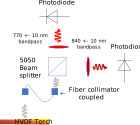
\includegraphics[width=0.8\textwidth]{\repodir/final/figures/schematics/output/PD_setup.png}
    \caption{Photodiode (PD) setup schematic. The acronyms are FCL: fiber coupled lens, BS: beam splitter, PB: bandpass filter, PD: photodiode, AMP: transimpedance amplifier, Osc.: Oscilloscope}
    \label{fig:SI_PD_setup_schematic}
\end{figure}



\begin{figure}[]
    \centering
    \includegraphics[width=0.8\textwidth]{\repodir/final/figures/setup_images/Photodiode_Setup.png}
    \caption{Image of the photodiode setup. Taken on 2023-05-24. }
    \label{fig:SI_PD_setup_image}
\end{figure}

\clearpage
\subsection{Emulsion Preparation and Delivery}

Potassium was introduced into the HVOF system using an emulsion of potassium carbonate (K2CO3) brine and kerosene (hereafter referred to as the "emulsion"). The emulsion was delivered into the HVOF fuel flow via a tee. The tee run carried the fuel flow while the tee branch accepted emulsion through a PTFE feed line which was served by a high-pressure syringe pump. The emulsion was loaded into three syringes in the syringe pump with the syringe outputs manifolded together. A switching valve allowed syringes to withdraw emulsion from the stirred reservoir or to infuse emulsion into the HVOF fuel line. Before igniting the torch, the 4.8 m emulsion line was filled to the tee to eliminate delay between initiating emulsion pumping and emulsion reaching the torch. At the tee, fuel flow momentum was used to mix the emulsion with the fuel flow over the 15cm distance between the tee and combustion chamber nozzle. 

Literature was reviewed for an emulsion specifically designed to work with brine — especially water-in-oil (W/O) emulsions. Developing emulsions for use in oilfields, Mohamed et al.\cite{mohamedInfluenceSurfactantStructure2017a} investigated high salinity W/O emulsions between “formation brine” and diesel. According to these authors, “[D]iesel and kerosene are used in the oilfields because of availability.” Their formation brine included more than 221,673 mg total dissolved solids (TDS) per liter of brine (~20\% by mass).  

We noted the most stable result in \cite{mohamedInfluenceSurfactantStructure2017a} and reproduced it using a K2CO3 brine, kerosene, and a SPAN 80 / TWEEN 80 surfactant blend meeting their recommended hydrophilic-lipophilic balance (HLB) of 6.8. The concentration of the surfactant was 0.5\% of the emulsion by volume - the minimum necessary found in \cite{mohamedInfluenceSurfactantStructure2017a} to obtain a stable emulsion. (Mohamed et al. measured that ~5\% of liquid came out of emulsion in 100 minutes at 120 °C).  

To generate the initial brine droplets, we used a spray nozzle. Spraying to create an emulsion is a standard practice used in this work because it avoids the temperature-rise associated with higher energy processes. \cite{atkinsonKeroseneEmulsionHow1890} These spray-generated droplets were then passed through an ultrasonic process to break them up further. This continuous process also minimized temperature rise because the material exited seconds after entering the ultrasonic field. 

%Broken citations above

\begin{enumerate}
    \item Prepare liquid components ahead of time, as follows:
    \begin{itemize}
        \item 100g supply of surfactant blend with HLB=6.8 by mixing 77g of Span 80 and 23g of Tween 80 on a magnetic stir plate 
        \item Eight aliquots of K2CO3 brine by mixing 847.7g of K2CO3 powder into 350mL of deionized water on a magnetic stirrer 
        \item Eight aliquots of prepared kerosene by mixing 5g of the surfactant blend into 106.5g of kerosene  
        \item Each Brine/Kerosene aliquot pair will produce 500mL of emulsion. 
    \end{itemize}

    \item Create a pre-emulsion:
    \begin{itemize}
        \item Decant an aliquot of prepared kerosene into a beaker and begin stirring on a magnetic stir plate. 
        \item Using a peristaltic pump, pump the aliquot of K2CO3 brine through a spray nozzle, producing a mist of droplets to fall into the prepared kerosene. Droplet/kerosene interfaces adsorb the surfactant to make a relatively fine pre-emulsion. 
    \end{itemize}

    \item Sonicate the pre-emulsion to create the final emulsion:
    \begin{itemize}
        \item While continuing to magnetically stir, pump the pre-emulsion through an ultrasonic continuous flow cell to further break up the dispersed brine droplets. 
        \item Batches were stored overnight and combined in magnetically stirred reservoir at the beginning of the photoionization experiment. 
    \end{itemize}
\end{enumerate}

Figure \ref{fig:SI_Emulsion_Process} shows a schematic of the emulsion preparation process outlined above. 


\begin{figure}[]
\centering
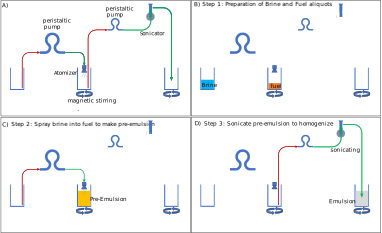
\includegraphics[width=0.9\textwidth]{\repodir/final/figures/schematics/output/Emulsion_Process.png}
\caption{Schematic of the emulsion preparation process. A) Overview of the emulsion preparation setup. B-D) Steps 1-3 of the emulsion preparation process.}
\label{fig:SI_Emulsion_Process}
\end{figure}


The emulsion recipe is given in Table \ref{tab:emulsion_parameters}. The mass of the fuel was incorrectly used as 109 g to calculate setpoints on each day except 2023-05-24, instead of 106.5 g. The emulsion recipe on 2023-05-24 corresponds to the physical emulsion prepared on each date, and is used in the calculation of process parameters including the potassium mass fraction, equivalence ratio, and total mass flow. 


\begin{table}[h]
\centering
\begin{tabular}{|l|l|l|}
\hline
\textbf{Parameter} & \textbf{2023-04-07 to 2023-05-18} & \textbf{2023-05-24} \\
\hline
$M_{K2CO3}$ & 84.7 gram & 84.7 gram \\
$M_{fuel}$ & 109.0 gram & 106.5 gram \\
$M_{water}$ & 350.0 gram & 350.0 gram \\
$M_{span80}$ & 3.84 gram & 3.84 gram \\
$M_{tween80}$ & 1.17 gram & 1.17 gram \\
$\rho_m$ & 1.056 gram / milliliter & 1.056 gram / milliliter \\
$M_{total}$ & 548.71 gram & 546.21 gram \\
$f_{fuel}$ & 0.19865 dimensionless & 0.19498 dimensionless \\
$f_{K2CO3}$ & 0.15436 dimensionless & 0.15507 dimensionless \\
\hline
\end{tabular}
\caption{Emulsion Recipe. M = mass, $rho_m$ is the measured mass density, $M_{total}$ is the calculated total mass, and $f_{fuel}$ and $f_{K2CO3}$ are the calculated mass fraction of fuel and $K_2CO_3$, respectively. The mass density ($\rho_m$) was measured by withdrawing a sample (about 10 ml) of emulsion and weighing it.  }


\label{tab:emulsion_parameters}
\end{table}
A representative picture of an emulsion batch is shown in \ref{fig:SI_Emulsion_Picture}, taken the day before the 2023-04-07 experiment. 

\begin{figure}[]
\centering
\includegraphics[width=0.8\textwidth]{\repodir/final/figures/setup_images/Emulsion_Picture_2023-04-07.png}
\caption{A picture of the potassium emulsion used on 2023-04-07. }
\label{fig:SI_Emulsion_Picture}
\end{figure}

\clearpage
\subsection{Additional pictures of experiment}

\begin{figure}[]
\centering
\includegraphics[width=0.8\textwidth]{\repodir/final/figures/setup_images/2023-05-18_Full_Setup_Topcam_2.png}
\caption{Full setup with top camera. Taken on 2023-05-18.}
\label{fig:SI_Full_Setup_Topcam}
\end{figure}

\begin{figure}[]
\centering
\includegraphics[width=0.8\textwidth]{\repodir/final/figures/setup_images/2023-05-24_PI_Setup.png}
\caption{Full view of experiment setup. Taken on 2023-05-24.}
\label{fig:SI_Full_Setup_PI}
\end{figure}

% final/figures/setup_images/2023-05-24_Rear_View.png

\begin{figure}[]
\centering
\includegraphics[width=0.8\textwidth]{\repodir/final/figures/setup_images/2023-05-24_Rear_View.png}
\caption{Rear view of experiment setup. Taken on 2023-05-24. The optical processing setup (beam splitter, filters, and photodiode) of the PD diagnostic can be seen on the table. }
\label{fig:SI_Rear_View}
\end{figure}

\begin{figure}[]
\centering
\includegraphics[width=0.8\textwidth]{\repodir/final/figures/setup_images/2023-05-18_Top_View.jpg}
\caption{Top view of experiment setup. Taken on 2023-05-18.}
\label{fig:SI_Top_View}
\end{figure}


